\chapter{Introduction}

%Channel limit
%
%URC
%Deep fade
%drop out
%5G





For all types of communication an important aspect is the channel through which the message is transmitted. For wireless communication, this is even more the case, as the channel changes constantly. The transmission of the message can be done in different environments, which have different impacts on the received signal. Common for all the environments is they introduce fading, which if not accounted for can have devastating effects for the transmission. 

Fading occurs when multipath propagation is present, that will introduce points in space where the waves adds either constructively or destructively, as can be seen on \autoref{intro_fading}. The constructive spots is not of much interest as it is only a couple of dB's difference, however the destructive interference can create spots with losses that borders minus infinite dB's. These spots are called deep fades and is is where the communication might suffer an outage. An outage occurs if the transmitted signal drops below the RX sensitivity level so the signal is lost. There are different tools to heighten the chance for the RX to receive signals that might experience deep fades and therefore increase the reliability of the communication link


\begin{figure}[H]
\centering
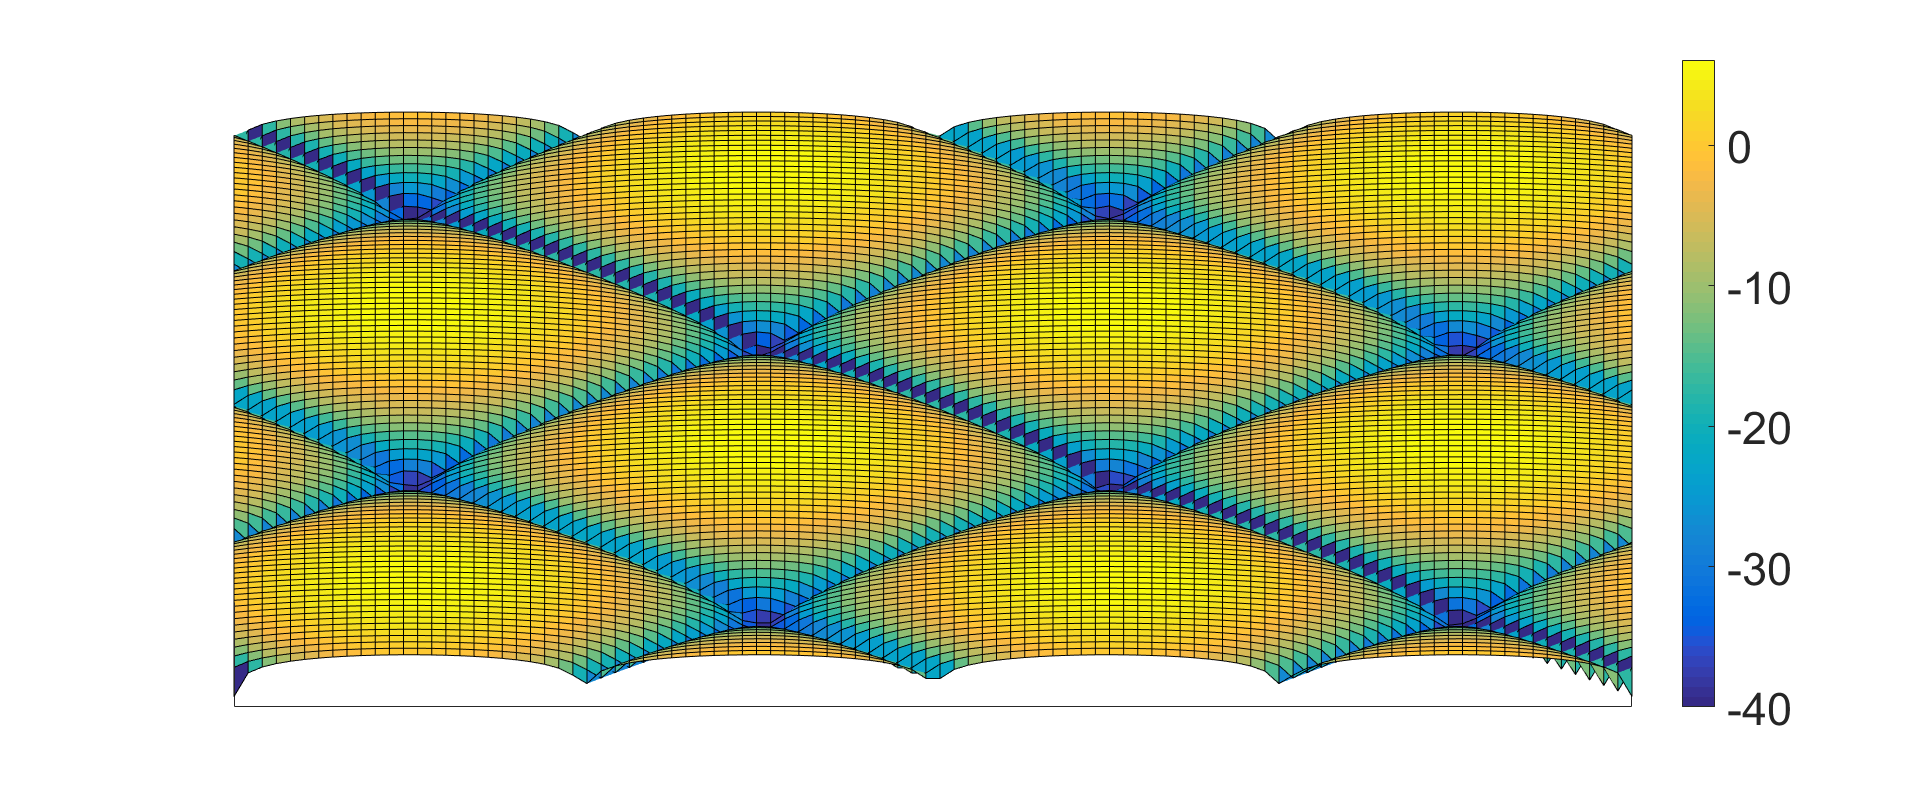
\includegraphics[width=\textwidth]{figures/intro_fading.png}
\caption{Fading gain from two wave fronts meeting, the deep fade spots have been elevated to allow for a better color resolution.}
\label{intro_fading}
\end{figure}

\section{Motivation}

The problem about fading is addressed already in cellular networks like \gls{LTE} or \gls{LTE-A} and many others, however with the development of the 5G network, new concepts is introduced. The 5G network is proposed to consist of three parts: \Gls{URLLC}, \gls{mMTC} and \gls{eMBB} \citep{5G}. Both the \gls{mMTC} and \gls{eMBB} will be sort of extensions to the existing networks, focusing on either the number of users or the data rate respectively, the \gls{URLLC} will introduce some new problems mostly wrt. the reliability where earlier networks have run with an outage probability of 0.1\%, the URLLC part shall have an outage probability under 0.001-0.0001\% \citep{LTE,Petar5G}, but also by lowering the latency from (>30 to <1) ms \citep{LTE,5G_Latency}. By introducing this new feature, critical system with special needs might be able to use the cellular network instead of a wired channel, which today provide a higher reliability, but comes with a greater cost both price and installation wise. Another problem is that future systems is predicted to need this feature \citep{Petar5G}. %By having a better reliability, there is a higher chance that some new application can be used on the cellular network. 
Some of the applications needing a URLLC channel could be self driving cars, in emergency cases, is it not only necessary to provide low latency, the certainty of the message to arrive is also desired. %where short message about position and speed can be send to other cars in the area, with low chance of needing re-transmission, which is importing in case of high alert situations. 

Other system that can gain advantages with URLLC, is systems where the communication window is very small and therefore do not have time for re-transmissions or a lot of data processing e.g. in error coding.


A problem about this is that to get this URLLC scenario, an in depth description of the channel is needed. A way to get higher reliability is to transmit with a higher power level, so there gets a higher \gls{SNR} on the communication link. But even if the overall signal is higher, there will still be problem with fading in some points in space as seen in \autoref{intro_fading}. Today descriptions of such channels have been verified to a probability level of around $10^{-3}$ - $10^{-4}$, any research for lower probability levels has assumed that an extrapolation of the models extend to probability levels that are multiple magnitudes lower as seen in \autoref{fading_gain}. Therefore this report wants to investigate this untested assumptions of multipath fading.

Problem statement:
Ascertain with 90\% confidence that in a multipath environment, the cumulative distribution function of the fading gain can be assumed to increase in a log log linear fashion between -60dB and -20dB.

To to this it is important to investigate the following points.

\begin{enumerate}
	\item Limit the 
	\item Find out how many samples needed for a set confidence interval of 90\%.
	\item Look into if there is a way to reduce the amount of samples needed by using statistical techniques.
	\item Figure out a measurement setup to achieve these sample numbers.
\end{enumerate}

\begin{figure}[H]
\centering
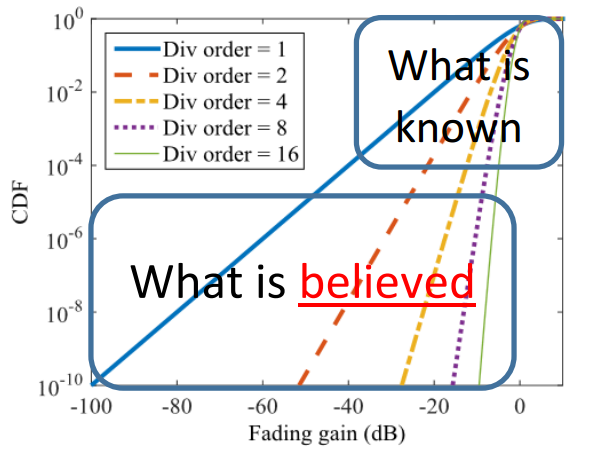
\includegraphics[width=0.65\textwidth]{figures/fading_gain.png}
\caption{\Gls{CDF} of fading gain in different channel environments.}
\label{fading_gain}
\end{figure}
\todo{source not just project description}

This might have been all right so far, but to achieve URLLC conditions, this the channel conditions need to be verified to those levels. That will be the focus of this project.


\section{Project outline}

As stated the focus will be to measure and compare channel characteristics at URLLC conditions. The project will not address the issue of low latency, as this is a completely different issue. This leaves a main aspects that needs investigation: The wireless channel and its practical limitations e.g. with a focus on fading. To investigate the channel, a test setup is needed, that can measure the varying signal power and therefore the limitations in the channel. This gives two main aspects for this project as seen on \autoref{ChannelAndEquip}.

\begin{figure}[H]
\centering
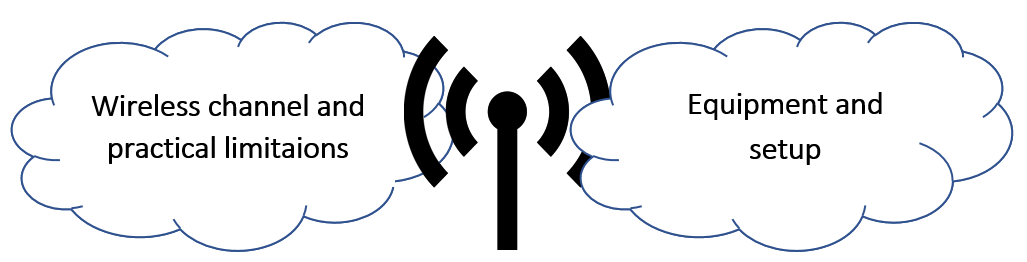
\includegraphics[width=0.85\textwidth]{figures/ProOutline.png}
\caption{Two of the main aspects of the project.}
\label{ChannelAndEquip}
\end{figure}



\begin{enumerate}
	\item 
	\item 
\end{enumerate}
 




